\chapter{Context}
\label{chap:context}

\section{Laboratoire de Mathématiques Informatique et Applications (LAMIA)}
\label{sec:lamia}

This project was done within the framework of the Master 2 Computer Science program at the
\textbf{Laboratoire de Mathématiques Informatique et Applications (LAMIA)} of the \textbf{Université des Antilles}.
The LAMIA is a research laboratory that is part of the Université des Antilles and is located in Guadeloupe. It focuses on the
intersection of mathematics, computer science, and their applications in various fields, including data science,
machine learning, and artificial intelligence. LAMIA conducts research that aims to advance theoretical understanding
and practical applications of mathematical and computational methods.

\section{Work Environment}
\label{sec:work_environment}

The following tools and technologies were used to develop algorithms and document the project:

\begin{itemize}
	\item \textbf{Python}: a programming language widely used in scientific computing, data analysis, and machine learning.
	\item \textbf{GitHub}: a version control platform for managing the source code.
	\item \textbf{GitHub Copilot}: for code completion.
	\item \textbf{Jupyter Notebook}: an interactive environment for writing and executing Python code, ideal for data analysis and
	      visualization.
	\item \textbf{Sklearn}: a Python library for machine learning that provides various algorithms and tools for data preprocessing,
	      model selection, and evaluation.
	\item \textbf{Pandas}: a Python library for data manipulation and analysis, providing data structures and functions for working with
	      structured data.
	\item \textbf{Matplotlib}: a Python library for graphics and data visualization, including 3D plotting capabilities.
	\item \LaTeX : a typesetting system used for writing technical and scientific documents.
	\item A personal computer running Windows 11 with a \textbf{Ryzen 7 6800H} processor and \textbf{32 GB} of RAM.
\end{itemize}

This internship was conducted within the office of the LAMIA with other students, which allowed for collaboration and
sharing of ideas and resources.

\section{Objectives}
\label{sec:objectives}

The main objective of this project is to explore and analyze genomic data, specifically the genomes of Tuberculosis (TB) strains, to
identify patterns and relationships between different strains. As well as to apply various data mining and data analysis techniques,
but also develop new methods and compare their performance to existing methods.

\chapter{Genomic data}
\label{chap:genomic_data}

Genomic data refers to the information contained in the DNA of an organism, which includes the sequences of nucleotides (Adenine, Thymine,
Cytosine, and Guanine). These are gathered through various methods, such as DNA sequencing, and can be used to study the genetic makeup
of organisms, identify genetic variations, and understand the relationships between different species. The Institute Pasteur has a large
collection of genomic data, including the genomes of various strains of Tuberculosis (TB), which is a major public health concern worldwide.

\section{Institut Pasteur}
\label{sec:institut_pasteur}

The Institut Pasteur is a renowned research institute located in Paris, France, dedicated to the study of biology,
microorganisms, diseases, and vaccines. Founded in 1887 by Louis Pasteur, the institute has played a pivotal role
in the development of modern microbiology and immunology. It is known for its contributions to the understanding of
infectious diseases and the development of vaccines, including those for rabies and tuberculosis. Founded by
Louis Pasteur in 1887, the Institut Pasteur has been at the forefront of scientific research and innovation for over
a century.

\section{The FASTA format}
\label{sec:fasta_format}

The FASTA format is a text-based format for representing nucleotide or protein
sequences~\textsuperscript{\cite{fasta-format-genbank,wikipedia-fasta-format-2025}}. It is widely used in bioinformatics
to store and exchange sequence data. A FASTA file consists of one or more sequences, each represented by a header line starting with
a greater-than symbol (\texttt{>}), followed by the sequence itself on the next line. The sequence codes for a protein who then codes for a
gene. The header line can contain additional information about the sequence, such as its identifier, description, or source. An example of a
FASTA file is shown in Figure~\ref{fig:fasta_example}.

\begin{center}
	\begin{figure}[H]
		\begin{BVerbatim}
			>sequence_id
			ATCGATCGATCGATCGATCGATCGATCG
			>sequence_id_2
			GCTAGCTAGCTAGCTAGCTAGCTAGCTA
			>sequence_id_3
			TAGCTAGCTAGCTAGCTAGCTAGCTAGC
			>sequence_id_4
			AGCTAGCTAGCTAGCTAGCTAGCTAGCT
			>sequence_id_5
			CATCGATCGATCGATCGATCGATCGATC
		\end{BVerbatim}
		\caption{Example of a FASTA file containing two sequences.}
		\label{fig:fasta_example}
	\end{figure}
\end{center}

The FASTA format is simple and easy to read, making it suitable for storing large amounts of sequence data. It is also compatible
with many bioinformatics tools and software, allowing for easy analysis and manipulation of sequence data.

\chapter{Clustering genomic data}
\label{chap:clustering_genomic_data}

\section{Preprocessing Genomic Data}
\label{sec:preprocessing_genomic_data}

Our data is a collection of Tuberculosis (TB) genomes, where each file contains the proteins and their respective nucleotide sequences
in FASTA format, for a total of 7057 files. These genomes were obtained from the \textbf{Institut Pasteur} and are part of the
\textbf{Mycobacterium tuberculosis complex} (MTBC), which is a group of closely related bacteria that cause TB. The goal is to cluster
these genomes based on their protein sequences and find ways to distinguish between different TB strains.

We started by creating a dataset containing the number of times each protein appears in each genome. This was done by
parsing the FASTA files and counting the occurrences of each protein sequence, we then removed the outliers, namely
"hypothetical proteins" and "putative proteins", which are not well characterized and do not provide useful information
for clustering. The resulting dataset is a CSV file of 7057 columns plus 1 column for the protein names and 2732 rows
plus 1 row for the header.

Considering the size of the dataset, we used Principal Component Analysis (PCA) set to 95\% variance to reduce the dimensionality
of the data while preserving as much variance as possible. PCA is a technique that transforms the data into a new coordinate
system, where the first principal component captures the maximum variance, the second captures the second maximum variance,
and so on.

We then calculated the silhouette score for different values of $k$, ranging from 2 to 10, to determine the optimal number
of clusters. The silhouette score was calculated using the `silhouette_score` function from the `sklearn.metrics` module,
which takes the data and the cluster labels as input. The optimal number of clusters is the one that maximizes the silhouette
score.

\subsection{First Results}
\label{subsec:first_results}

The initial results showed that the silhouette score was highest for $k=9$, indicating that this was the optimal number of clusters.
However, the clusters were not well separated, or some points are isolated in their cluster, as seen in Figure~\ref{fig:clusters_k9_pca},
which suggests that the data may not be well suited for clustering with K-means, or that the features used for clustering are not
informative enough. We also tried without applying PCA but achieved similar results. We also observed fewer clusters, as seen in
Figure~\ref{fig:clusters_k9_no_PCA}.

After reviewing the data, we found that there is significant overlap between the points, so we switched to 3D visualization to better
understand the clusters. With Figure~\ref{fig:clusters_k9_pca_3d} and Figure~\ref{fig:clusters_k9_no_PCA_3d}, we can see that the
clusters are still not well separated, but we can conclude that a 2D space was not appropriate for visualizing the clusters.

These results suggest that K-means clustering may not be the best approach for this dataset, or that the data may need further or a
different preprocessing step to improve the clustering results. We will explore alternative clustering algorithms in the next section.

\begin{figure}[H]
	\centering
	\begin{minipage}[t]{0.48\textwidth}
		\centering
		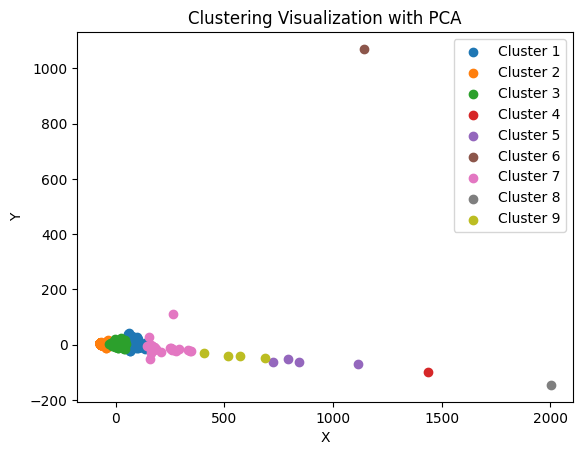
\includegraphics[width=0.95\textwidth]{../imgs/graphs/clustering/cluster_pca.png}
		\caption{Clusters obtained with K-means clustering after applying PCA.}
		\label{fig:clusters_k9_pca}
	\end{minipage}\hfill
	\begin{minipage}[t]{0.48\textwidth}
		\centering
		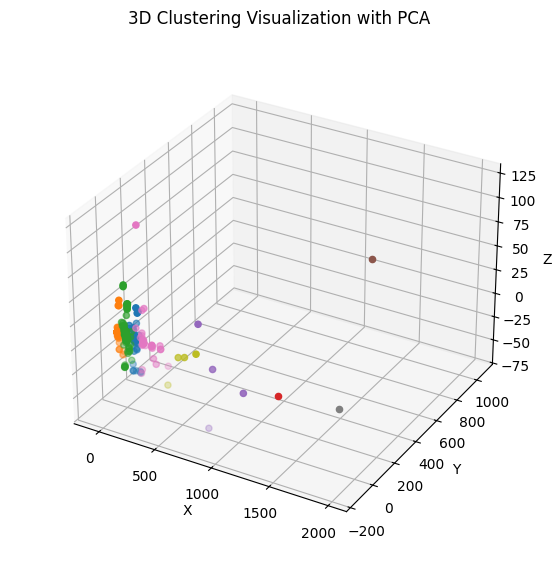
\includegraphics[width=0.95\textwidth]{../imgs/graphs/clustering/cluster_pca_3d.png}
		\caption{Clusters obtained with K-means clustering after applying PCA in 3D.}
		\label{fig:clusters_k9_pca_3d}
	\end{minipage}
\end{figure}

\begin{figure}[H]
	\centering
	\begin{minipage}[t]{0.48\textwidth}
		\centering
		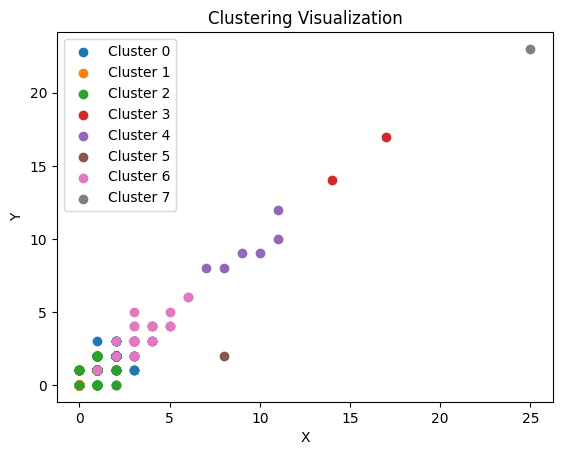
\includegraphics[width=0.95\textwidth]{../imgs/graphs/clustering/cluster_nopca.png}
		\caption{Clusters obtained with K-means clustering without applying PCA.}
		\label{fig:clusters_k9_no_PCA}
	\end{minipage}\hfill
	\begin{minipage}[t]{0.48\textwidth}
		\centering
		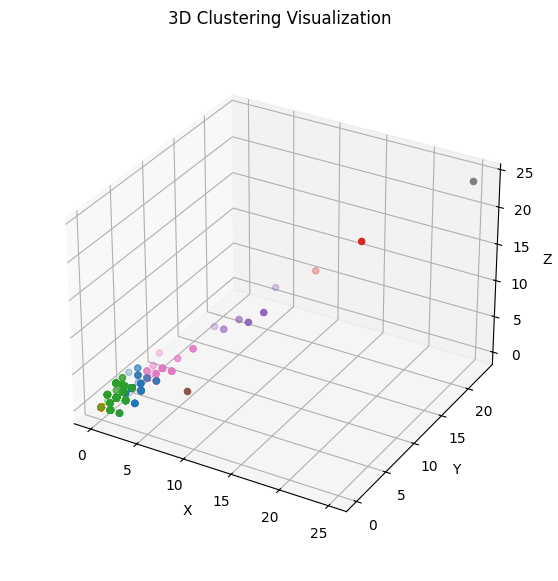
\includegraphics[width=0.95\textwidth]{../imgs/graphs/clustering/cluster_nopca_3d.png}
		\caption{Clusters obtained with K-means clustering without applying PCA in 3D.}
		\label{fig:clusters_k9_no_PCA_3d}
	\end{minipage}
\end{figure}

\section{New Approach using DBSCAN and HDBSCAN}
\label{subsec:new_approach_dbscan_hdbscan}

To address the poor clustering results obtained with K-means, we explored alternative clustering algorithms, specifically
\textbf{DBSCAN} and \textbf{HDBSCAN}.

DBSCAN (Density-Based Spatial Clustering of Applications with Noise) is a density-based clustering algorithm that
groups points that are close together based on a distance measurement and a minimum number of points. It is particularly
effective for datasets with varying densities and can identify noise points that do not belong to any cluster.

HDBSCAN (Hierarchical Density-Based Spatial Clustering of Applications with Noise) is an extension of DBSCAN that builds
a hierarchy of clusters and allows for more flexible clustering by varying the density threshold. It can also handle varying
cluster shapes and sizes.

\subsection{Results}
\label{subsec:results_dbscan_hdbscan}

During our testing, we applied both DBSCAN and HDBSCAN with an epsilon value of 1 and a minimum number of samples of 5.
These techniques were both applied to the dataset with and without PCA. We can see from Figure~\ref{fig:clusters_dbscan_no_pca}
to Figure~\ref{fig:clusters_hdbscan_pca_3d} that the clusters obtained with DBSCAN and HDBSCAN are more just a bit more
discernible than those obtained with K-means clustering. But the clusters are still closely packed together, we can conclude
that the problem lies with the way the dataset was created. A similar observation can be made when not applying PCA, as shown
in Figure~\ref{fig:clusters_dbscan_no_pca} to Figure~\ref{fig:clusters_hdbscan_no_pca_3d} in the appendix.

\begin{figure}[H]
	\centering
	\begin{minipage}[t]{0.48\textwidth}
		\centering
		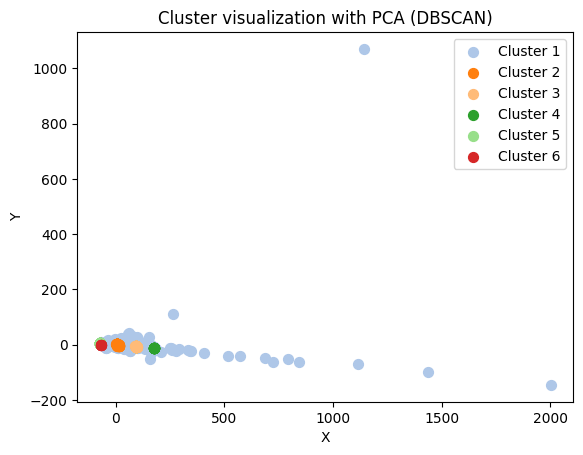
\includegraphics[width=0.95\textwidth]{../imgs/graphs/clustering/dbscan_pca.png}
		\caption{Clusters obtained with DBSCAN after applying PCA.}
		\label{fig:clusters_dbscan_pca}
	\end{minipage}\hfill
	\begin{minipage}[t]{0.48\textwidth}
		\centering
		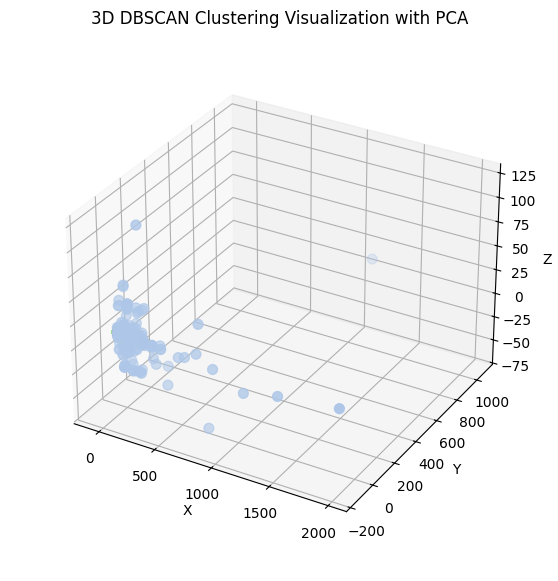
\includegraphics[width=0.95\textwidth]{../imgs/graphs/clustering/dbscan_pca_3d.png}
		\caption{Clusters obtained with DBSCAN after applying PCA in 3D.}
		\label{fig:clusters_dbscan_pca_3d}
	\end{minipage}
\end{figure}

\begin{figure}[H]
	\centering
	\begin{minipage}[t]{0.48\textwidth}
		\centering
		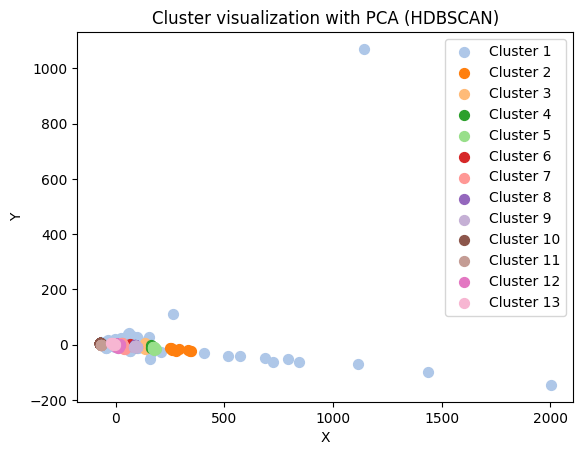
\includegraphics[width=0.95\textwidth]{../imgs/graphs/clustering/hdbscan_pca.png}
		\caption{Clusters obtained with DBSCAN after applying PCA.}
		\label{fig:clusters_hdbscan_pca}
	\end{minipage}\hfill
	\begin{minipage}[t]{0.48\textwidth}
		\centering
		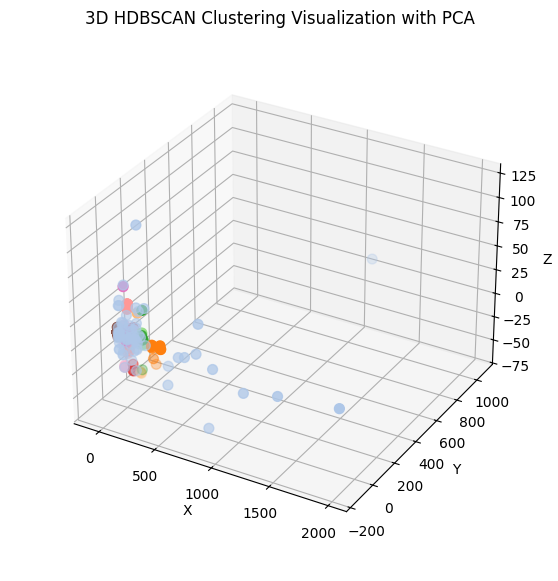
\includegraphics[width=0.95\textwidth]{../imgs/graphs/clustering/hdbscan_pca_3d.png}
		\caption{Clusters obtained with DBSCAN after applying PCA in 3D.}
		\label{fig:clusters_hdbscan_pca_3d}
	\end{minipage}
\end{figure}

\section{Trying an autoencoder}
\label{sec:autoencoder}

To further explore the clustering of the genomic data, we decided to try an autoencoder. After getting the embeddings from the autoencoder,
we applied the K-means clustering algorithm to the encoded data. We can see in Figure~\ref{fig:clusters_autoencoder} and
Figure~\ref{fig:clusters_autoencoder_3d} that the clusters obtained with K-means clustering on the encoded data are more discernible
than those obtained with K-means clustering on the original data. However, we observe a great intra-cluster distance, which suggests that
the autoencoder may not have learned a good data representation, or that the dataset or features were not well suited for clustering.

\begin{figure}[H]
	\centering
	\begin{minipage}[t]{0.48\textwidth}
		\centering
		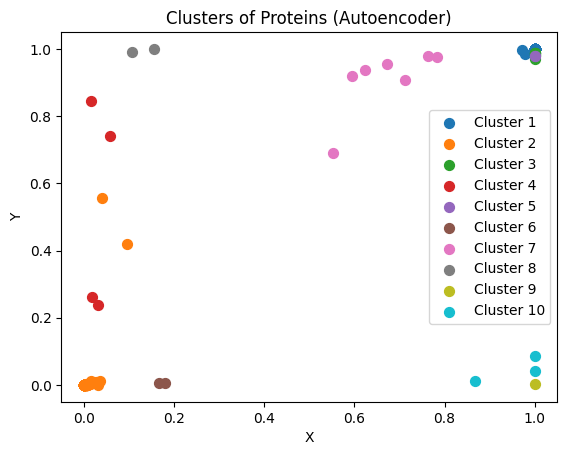
\includegraphics[width=0.95\textwidth]{../imgs/graphs/clustering/kmeans_autoencoder.png}
		\caption{Clusters obtained with K-means clustering on the encoded data.}
		\label{fig:clusters_autoencoder}
	\end{minipage}\hfill
	\begin{minipage}[t]{0.48\textwidth}
		\centering
		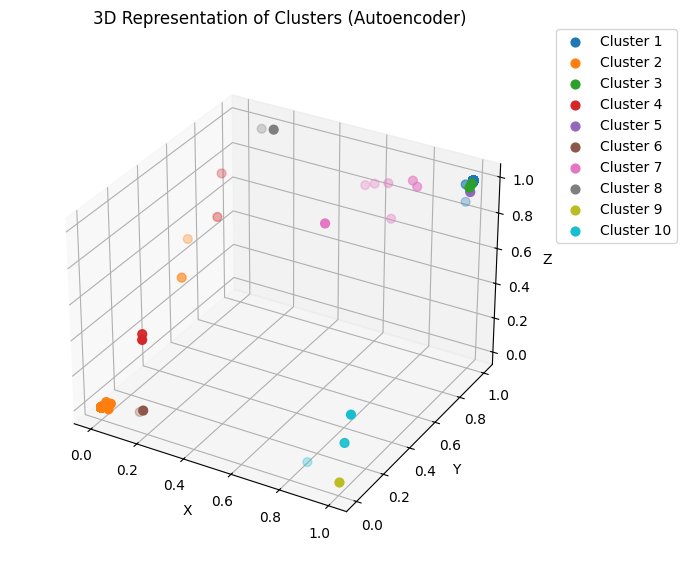
\includegraphics[width=0.95\textwidth]{../imgs/graphs/clustering/kmeans_autoencoder_3d.png}
		\caption{Clusters obtained with K-means clustering on the encoded data in 3D.}
		\label{fig:clusters_autoencoder_3d}
	\end{minipage}
\end{figure}

\chapter{Using CNNs to identify TB Strains}
\label{chap:cnn_tb_strains}

The clustering approach did not yield satisfactory results, so we decided to explore a different approach by converting the genomic
data into images. This approach allows us to leverage the power of Convolutional Neural Networks (CNNs) to classify the images and
identify the TB strains. These images are generated from the genomic data by applying five metrics to the nucleotide sequences,
which are then converted into pixel values. The pixel value is determined by a combination of three metrics, resulting in
ten different combinations of metrics, each represented by a different color channel in the image (Red, Green and Blue, RGB).
The resulting images can be used to train a CNN to classify the TB strains based on their genomic data. This approach has the
potential to improve the classification accuracy and provide a more robust method for identifying TB strains.

\section{Building the dataset}
\label{sec:building_dataset}

As mentioned earlier, each genome was converted into an image where each pixel is determined by a combination of three metrics of
following metrics:

\begin{itemize}
	\item \textbf{Chargaff} index~\textsuperscript{\cite{Clarke-Hurst-2006}}: provides the fraction of nucleic bases G and C of the sequence.
	      The formula is:
	      \begin{equation}
		      100 \times \frac{Gcount + Ccount}{Sequence\_size}
	      \end{equation}
	\item \textbf{Component} index~\textsuperscript{\cite{Mrazek-Karlin-1998}}: evaluates the distribution of the bases in a sequence
	      by comparing the number of each base A and T to the expected frequency of those bases in a balanced distribution. The formula is:
	      \begin{equation}
		      \frac{(Acount + Tcount) + \frac{Sequence\_size}{2}}{\frac{Sequence\_size}{2}}
	      \end{equation}
	\item \textbf{Diversity} index~\textsuperscript{\cite{Peregrin-Alvarez-Parkinson-2007}}: measures the diversity of bases in a sequence
	      by comparing the number of different subsequences of a given size to the expected frequency of those subsequences in a balanced
	      distribution. The formula is:
	      \begin{equation}
		      \frac{Number\textsubscript{unique subsequences}}{Expected\textsubscript{subsequences frequency}}
	      \end{equation}
	\item \textbf{Skew} index~\textsuperscript{\cite{Arakawa-Tomita-2007}}: measures the asymmetry of the distribution of nucleobases in
	      a sequence. The formula is:
	      \begin{equation}
		      \frac{(Gcount - Ccount)}{Sequence\_size}
	      \end{equation}
	\item \textbf{Nuclescore} index~\textsuperscript{\cite{Moco-et-al-2022}}: empirical measure that combines multiple metrics from a genome sequence to synthesize the nucleotide
	      information of a genome in order to differentiate species based only on their sequences. The formula is:
	      \begin{equation}
		      \log_{2}(\frac{Variance \times GC\textsubscript{ratio} \times AT\textsubscript{count}/GC\textsubscript{ratio}}{\sqrt{Sequence\_size}})
	      \end{equation}
\end{itemize}

We get ten combinations of these metrics, each represented by a different color channel in the image after being normalized to the range [0, 255].
This conversion is applied at different resolutions, from 4px (2x2) to 100px (10x10), but for the training, all images were resized to a 32x32px resolution.
The resulting images put into their corresponding class based on the strain they belong to, as shown in Figure~\ref{fig:example_image}. We have the following
classes:

\begin{itemize}
	\item \textbf{M} with 185 samples.
	\item \textbf{East Asian} with 1651 samples.
	\item \textbf{East-African Indian} with 267 samples.
	\item \textbf{Euro-American} with 4409 samples.
	\item \textbf{Indo-Oceanic} with 259 samples.
\end{itemize}

We also made mosaic images by combining the corresponding images from each combination of metrics resulting in a 5x2 grid rectangular image as shown
in Figure~\ref{fig:mosaic_example}. We chose a 5x2 grid because it creates complete images without any empty pixels, which is important for the
training of the CNN. The images are also resized to a 20x50px resolution for training.

\begin{figure}[H]
	\centering
	\begin{minipage}[t]{0.48\textwidth}
		\centering
		\includegraphics[width=0.4\textwidth]
		{../scripts/img_analysis/train-raw/arrays/100px/Chargaff-Composante-Diversite/_M_/GCF_000010685.1_ASM1068v1_genomic.fna.ffn_M_100px_Chargaff-Composante-Diversite.png}
		\caption{Example of an image generated from the genome of a TB strain using the Chargaff, Component and Diversity metrics at 100px resolution.}
		\label{fig:example_image}
	\end{minipage}\hfill
	\begin{minipage}[t]{0.48\textwidth}
		\centering
		\includegraphics[width=0.95\textwidth]{../scripts/img_analysis/test-raw/mosaics/100px/_M_/GCF_000666425.1_Myco_afri_MAL010100_V1_genomic.fna.ffn_M_100px_mozaic.png}
		\caption{Example of a mosaic image obtained from the individual images at 100px resolution.}
		\label{fig:mosaic_example}
	\end{minipage}
\end{figure}


\subsection{Initial testing}
\label{subsec:initial_testing}

The resulting dataset is highly imbalanced, with some classes having significantly more samples than others. This can lead to biased models
that perform poorly on minority classes. We decided to train our CNN on the dataset as-is, without any preprocessing or balancing techniques,
to see how it performs on the imbalanced dataset. For the sake of brevity, we will only present the results for the combination of Chargaff,
Composition and Diversity metrics at 100px resolution, for the mosaic images we will present the results for the 100px resolution as well.

\subsubsection{Results}
\label{subsubsec:results_initial_testing}

As shown in Figure~\ref{fig:cnn_validation_accuracy_std}, the 4px images yielded the worst performance, with a validation accuracy between 66\%
and 76\%. We then observed a significant improvement in performance as the resolution increases with the accuracy starting to stabilize
around 92\% and 94\% starting from the 36px resolution. Figure~\ref{fig:cnn_confusion_matrix_100px_std} and Table~\ref{tab:performance_metrics_100px_std}
show that the overall performances of the model are good, except for the East-African Indian and Indo-Oceanic classes with more moderate performances.

East-African Indian shows a moderate recall of 0.779 and a precision of 0.904, indicating that the model is able to correctly classify
most of the samples in this class, but it also misclassifies some samples as other classes. The Indo-Oceanic class has a recall of 0.988,
indicating that the model is able to correctly classify most of the samples in this class, but it has a lower precision of 0.718, indicating
that the model misclassifies some samples as this class.

\begin{figure}[H]
	\centering
	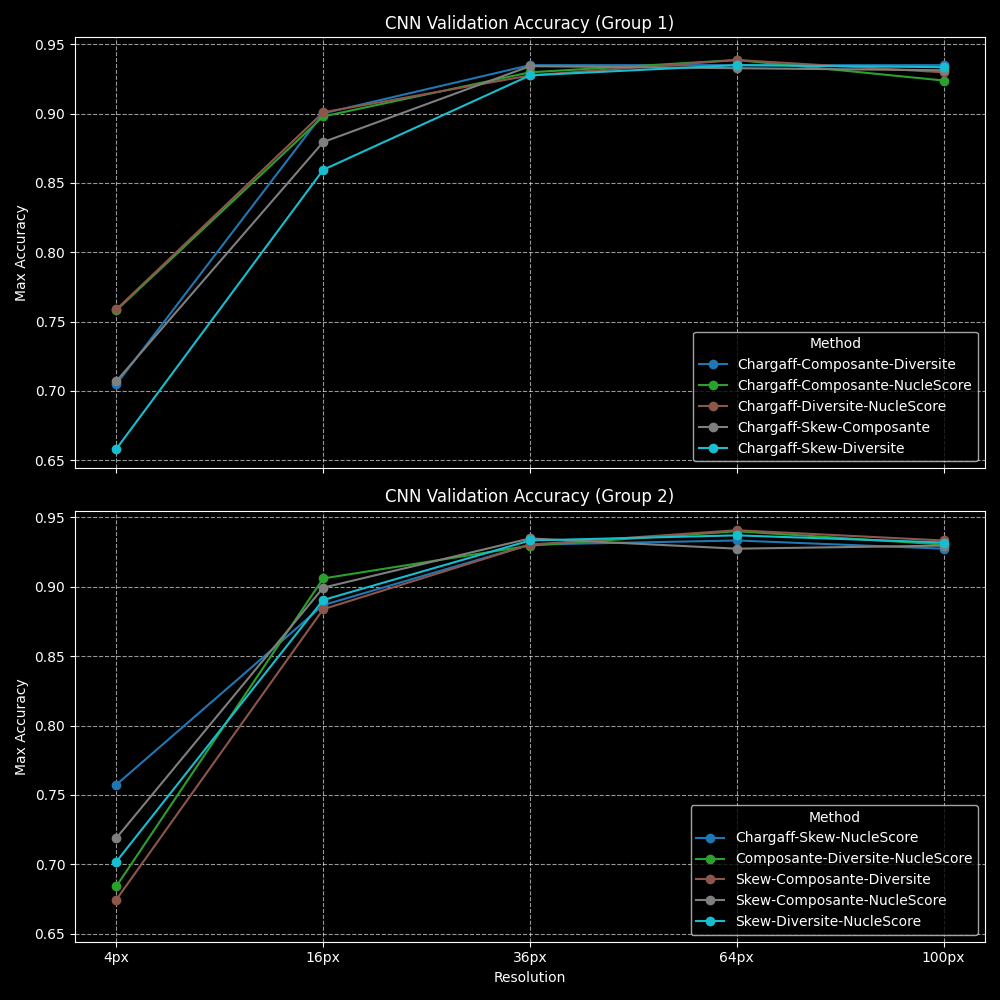
\includegraphics[width=0.6\textwidth]{../imgs/graphs/standard/cnn_validation_accuracy_groups_mask_5_std.png}
	\caption{Graph showing the validation accuracy of the model on the different methods at 100px resolution without any preprocessing or
		balancing techniques applied.}
	\label{fig:cnn_validation_accuracy_std}
\end{figure}

\begin{figure}[H]
	\centering
	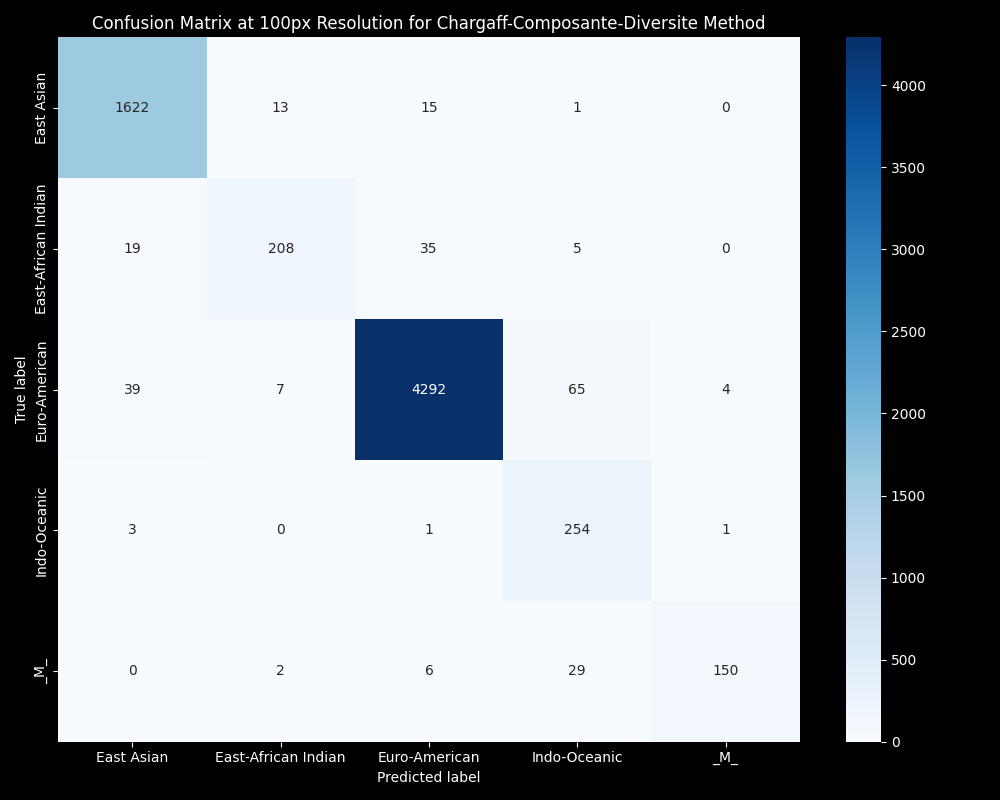
\includegraphics[width=0.65\textwidth]{../imgs/graphs/standard/cnn_confusion_matrix_100px_mask_5_std-old.png}
	\caption{Confusion matrix of the model on the images obtained from the Chargaff-Component-Diversity combination at 100px resolution without any
		preprocessing or balancing techniques applied.}
	\label{fig:cnn_confusion_matrix_100px_std}
\end{figure}

\begin{table}[H]
	\centering
	\begin{tabular}{|c|c|c|c|c|}
		\hline
		\textbf{Class}      & \textbf{Precision} & \textbf{Recall} & \textbf{Specificity} & \textbf{Accuracy} \\
		\hline
		East Asian          & 0.965              & 0.982           & 0.988                & 0.987             \\
		East-African Indian & 0.904              & 0.779           & 0.997                & 0.988             \\
		Euro-American       & 0.987              & 0.974           & 0.976                & 0.975             \\
		Indo-Oceanic        & 0.718              & 0.988           & 0.985                & 0.985             \\
		M                   & 0.968              & 0.802           & 0.999                & 0.994             \\
		\hline
	\end{tabular}
	\caption{Performance metrics of the model on the images obtained from the Chargaff-Component-Diversity combination at 100px resolution without any
		preprocessing or balancing techniques applied.}
	\label{tab:performance_metrics_100px_std}
\end{table}

For the mosaic images, we observed similar results, with the model achieving a validation accuracy of around 95\% at 100px resolution. While most of the metrics
are similar to the individual images, the East-African Indian class improved its recall, the precision dropped to 0.662. This indicates that, while the model is able to
correctly classify most of the samples in this class, other classes are confused with this class.

\begin{table}[H]
	\centering
	\begin{tabular}{|c|c|c|c|c|}
		\hline
		\textbf{Class}      & \textbf{Precision} & \textbf{Recall} & \textbf{Specificity} & \textbf{Accuracy} \\
		\hline
		East Asian          & 0.976              & 0.970           & 0.992                & 0.987             \\
		East-African Indian & 0.662              & 0.858           & 0.982                & 0.977             \\
		Euro-American       & 0.991              & 0.963           & 0.984                & 0.970             \\
		Indo-Oceanic        & 0.771              & 0.973           & 0.988                & 0.988             \\
		M                   & 0.966              & 0.908           & 0.999                & 0.997             \\
		\hline
	\end{tabular}
	\caption{Performance metrics of the model on the mosaic images at 100px resolution without any preprocessing or balancing techniques applied.}
	\label{tab:performance_metrics_mosaic_std}
\end{table}

Overall, this model shows good performance on the imbalanced dataset, but there is still room for improvement. But we will explore different techniques
to address the class imbalance issue in the following sections.

\section{Mitigating class imbalance}
\label{sec:mitigating_class_imbalance}

We have multiple ways of addressing the class imbalance issue in our dataset, including:

\begin{itemize}
	\item Cross validation
	\item Under-sampling
	\item Data augmentation
	\item Combining under-sampling and data augmentation
\end{itemize}

We will explore each of these techniques in the following sections and compare the results to see which one yields the best performance.

\subsection{Cross validation}
\label{subsec:cross_validation}

Cross validation is a technique used to evaluate the performance of a model by splitting the dataset into multiple subsets, or folds.
The model is trained on a subset of the data and tested on the remaining data, and this process is repeated for each fold.
This allows for a more robust evaluation of the model's performance, as it reduces the risk of overfitting to a specific subset of the data.

\subsubsubsection{Remaking the dataset}
\label{subsubsec:remaking_dataset}

During our testing, we realized that we were testing our model with images the model was trained on, which is not a good practice. We decided to
split our dataset into a training set and a test set, with 90\% of the samples in the training set and 10\% in the test set. The files are separated
into two folders to avoid any overlap between the training and test sets.

\subsubsection{Results}
\label{subsec:results_cross_validation}

During our testing, we used the K-fold cross validation technique with 5 folds with 15 epochs and a batch size of 32. We observed that the model
was able to achieve a validation accuracy of around 96\% during validation for all of 10 combinations of the metrics at 100px resolution, as shown in
Figure~\ref{fig:kfold_accuracy}. The confusion matrix in Figure~\ref{fig:kfold_confusion_matrix} shows that the model was able to correctly classify
most of the samples, with only a few misclassifications.

With Table~\ref{tab:kfold_performance_metrics} we can see that the model has good performance across most classes. Surprisingly enough, the M class,
which has the least number of samples, has better performance than the East-African Indian class, which has more samples. This suggests that the model
is able to generalize well to the minority classes, even with the class imbalance issue.

For the mosaic images, we applied the same k-fold cross validation technique with 5 folds and 15 epochs, and we observed similar results compared to the
individual images. The East-African Indian class has a slightly lower precision but a slightly higher recall, indicating that the model is able to
correctly classify most of the samples in this class, but it also misclassifies some samples as other classes. The Indo-Oceanic class has a recall of 1,
indicating that the model was able to correctly classify all the samples in this class, but it has a lower precision of 0.684, indicating that the model
misclassifies some samples as this class. Specificity and accuracy are nearly the same as the individual images, as shown in
Table~\ref{tab:kfold_performance_metrics_mosaic}.

\begin{figure}[H]
	\centering
	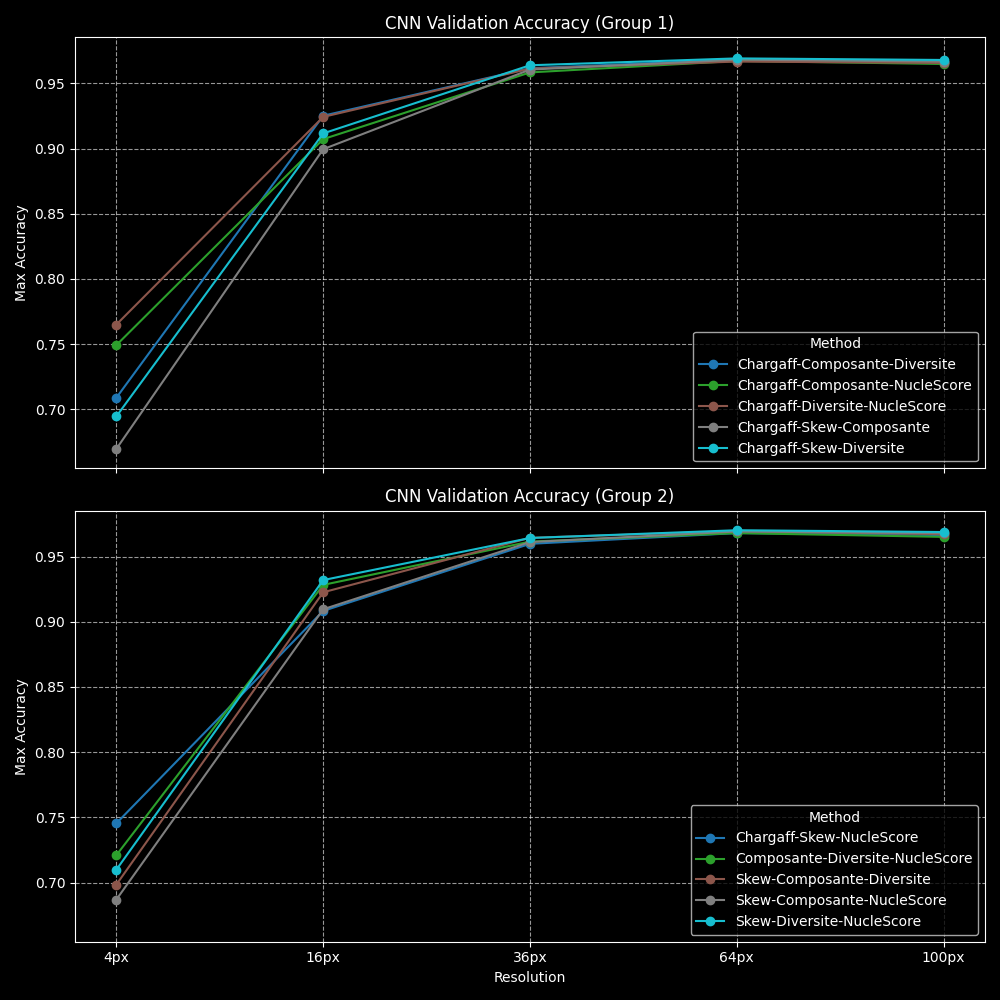
\includegraphics[width=0.65\textwidth]{../imgs/graphs/kfold/cnn_validation_accuracy_groups_mask_5_kfold_std.png}
	\caption{Graph showing the validation accuracy of the CNN model with k-fold cross validation applied on the different methods.}
	\label{fig:kfold_accuracy}
\end{figure}

\begin{figure}[H]
	\centering
	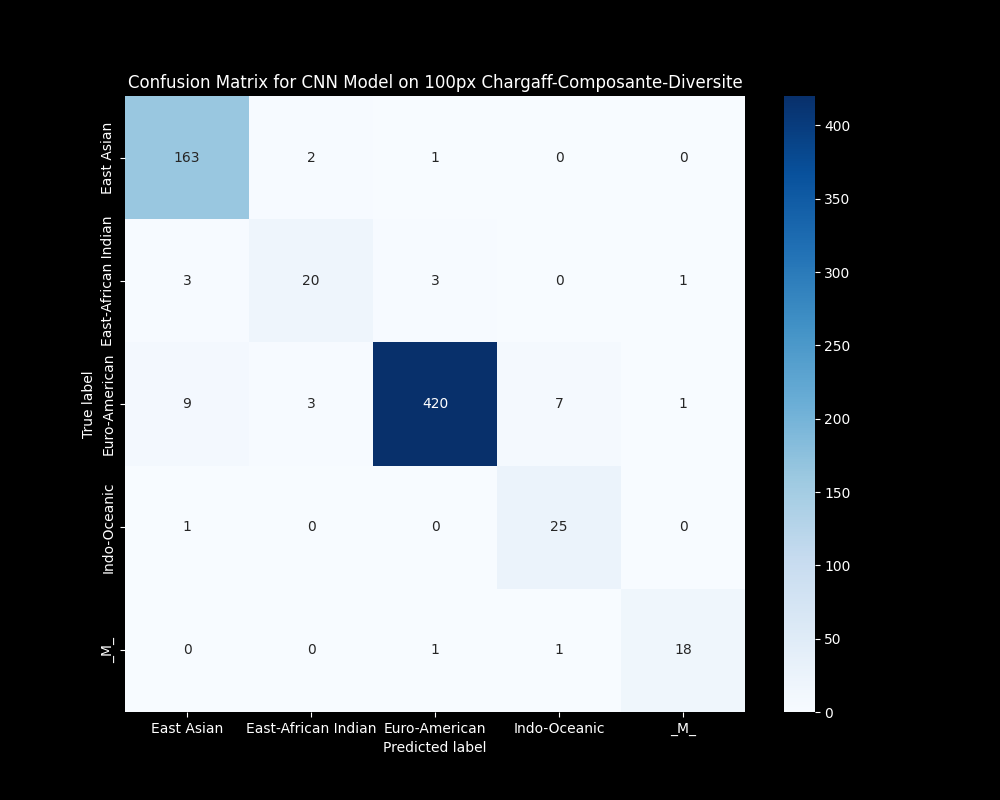
\includegraphics[width=0.65\textwidth]{../imgs/graphs/kfold/cnn_confusion_matrix_100px_mask_5-kfold_std.png}
	\caption{Confusion matrix of the CNN model with k-fold cross validation applied on the images obtained from the Chargaff-Component-Diversity
		combination at 100px resolution.}
	\label{fig:kfold_confusion_matrix}
\end{figure}

\begin{table}[H]
	\centering
	\begin{tabular}{|c|c|c|c|c|}
		\hline
		\textbf{Class}      & \textbf{Precision} & \textbf{Recall} & \textbf{Specificity} & \textbf{Accuracy} \\
		\hline
		East Asian          & 0.926              & 0.982           & 0.975                & 0.976             \\
		East-African Indian & 0.800              & 0.741           & 0.992                & 0.982             \\
		Euro-American       & 0.988              & 0.955           & 0.979                & 0.963             \\
		Indo-Oceanic        & 0.758              & 0.962           & 0.988                & 0.987             \\
		M                   & 0.900              & 0.900           & 0.997                & 0.994             \\
		\hline
	\end{tabular}
	\caption{Performance metrics with k-fold cross validation applied on the images obtained from the Chargaff-Component-Diversity
		combination at 100px resolution.}
	\label{tab:kfold_performance_metrics}
\end{table}


\begin{table}[H]
	\centering
	\begin{tabular}{|c|c|c|c|c|}
		\hline
		\textbf{Class}      & \textbf{Precision} & \textbf{Recall} & \textbf{Specificity} & \textbf{Accuracy} \\
		\hline
		East Asian          & 0.932              & 0.988           & 0.977                & 0.979             \\
		East-African Indian & 0.724              & 0.778           & 0.988                & 0.979             \\
		Euro-American       & 0.995              & 0.945           & 0.992                & 0.962             \\
		Indo-Oceanic        & 0.684              & 1.000           & 0.982                & 0.982             \\
		M                   & 0.944              & 0.850           & 0.998                & 0.994             \\
		\hline
	\end{tabular}
	\caption{Performance metrics with k-fold cross validation applied on the mosaic images at 100px resolution.}
	\label{tab:kfold_performance_metrics_mosaic}
\end{table}

The performances of the model with cross validation are close to the ones obtained without cross validation. It seems to perform slightly
better, but the difference is not significant enough to conclude that cross validation improves the performance of the model. However, it is
important to note that cross validation is a good practice to evaluate the performance of a model, as it reduces the risk of overfitting
to a specific subset of the data and provides a more robust evaluation of the model's performance.

\subsection{Under-sampling}
\label{subsec:under_sampling}

Under-sampling is a technique used to address the class imbalance issue by reducing the number of samples in the majority classes. In our
application, we decided to reduce the number of samples in the Euro-American and East Asian classes to a total of 1000 samples each, while keeping
the other classes unchanged. This was done to balance the dataset and ensure that the model is not biased towards the majority classes.

\subsubsubsection{Results}
\label{subsubsec:results_under_sampling}

This time we observe a drop in the validation accuracy of the model (Figure~\ref{fig:under_sampling_accuracy}) compared to the previous results,
with the accuracy being between 89\% and 93\% for the 100px resolution. There is also a significant drop in the performance of the model
on the East-African Indian class, while the recall slightly improves, the precision drops significantly, indicating that the model identify
other classes as East-African Indian. This is likely due to the reduced number of samples in the Euro-American and East Asian classes,
which may have led to a less representative training set for these classes. It can be seen in Figure~\ref{fig:under_sampling_confusion_matrix}
and Table~\ref{tab:under_sampling_performance_metrics}.

\begin{table}[H]
	\centering
	\begin{tabular}{|c|c|c|c|c|}
		\hline
		\textbf{Class}      & \textbf{Precision} & \textbf{Recall} & \textbf{Specificity} & \textbf{Accuracy} \\
		\hline
		East Asian          & 0.964              & 0.982           & 0.988                & 0.987             \\
		East-African Indian & 0.571              & 0.889           & 0.972                & 0.969             \\
		Euro-American       & 0.998              & 0.936           & 0.996                & 0.957             \\
		Indo-Oceanic        & 0.765              & 1.000           & 0.988                & 0.988             \\
		M                   & 0.905              & 0.950           & 0.997                & 0.996             \\
		\hline
	\end{tabular}
	\caption{Performance metrics with under-sampling applied on the images obtained from the Chargaff-Component-Diversity
		combinations at 100px resolution.}
	\label{tab:under_sampling_performance_metrics}
\end{table}

For the mosaic images, we observe an even more significant drop in the precision of the East-African Indian class, which drops to 0.361 from
0.724 with cross validation on these images (Figure~\ref{tab:under_sampling_performance_metrics_mosaic}). The model misclassifies a lot of
Euro-American samples as East-African Indian, more than there are actual East-African Indian samples in the dataset
(Figure~\ref{fig:under_sampling_mosaic_confusion_matrix}).

\begin{table}[H]
	\centering
	\begin{tabular}{|c|c|c|c|c|}
		\hline
		\textbf{Class}      & \textbf{Precision} & \textbf{Recall} & \textbf{Specificity} & \textbf{Accuracy} \\
		\hline
		East Asian          & 0.952              & 0.952           & 0.984                & 0.976             \\
		East-African Indian & 0.361              & 0.815           & 0.940                & 0.935             \\
		Euro-American       & 0.992              & 0.893           & 0.987                & 0.926             \\
		Indo-Oceanic        & 0.765              & 1.000           & 0.988                & 0.988             \\
		M                   & 0.864              & 0.950           & 0.995                & 0.994             \\
		\hline
	\end{tabular}
	\caption{Performance metrics with under-sampling applied on the mosaic images at 100px resolution.}
	\label{tab:under_sampling_performance_metrics_mosaic}
\end{table}

Instead of improving the performance of the model like we hoped, under-sampling led to a drop in the performance of the model, especially
on the East-African Indian class. Still, even with the lowest number of samples, the M class keeps stable metrics. We're still unsure why
this is the case, but it could be due to the fact that the M class has a very distinct pattern that the model can pick up on, even with
a reduced number of samples.

\subsection{Data augmentation}
\label{subsec:data_augmentation}

For this test, we use the SMOTE-generated images to increase the number of samples in the minority classes, East-African Indian, Indo-Oceanic and M,
the other classes are kept unchanged. The aforementioned classes are augmented so that the resulting number of samples contains 25\% of generated images
for each class.

\subsubsubsection{Results}
\label{subsubsec:results_data_augmentation}

With data augmentation, we once again observe similar behavior for the East-African Indian and Indo-Oceanic classes between the individual and mosaic images.
The individual images seem to yield a better precision metric for the Indo-Oceanic class (Table~\ref{tab:augmentation_performance_metrics}), while the mosaic
images favors the East-African Indian class (Table~\ref{tab:augmentation_performance_metrics_mosaic}) in that regard. But this time, those two classes are
roughly on par with each other, with metrics that are close, if not slightly better than with cross validation. This technique seems to be promising, as it
allows us to increase the number of samples in the minority classes while keeping the majority classes unchanged.

\begin{table}[H]
	\centering
	\begin{tabular}{|c|c|c|c|c|}
		\hline
		\textbf{Class}      & \textbf{Precision} & \textbf{Recall} & \textbf{Specificity} & \textbf{Accuracy} \\
		\hline
		East Asian          & 0.976              & 0.976           & 0.992                & 0.988             \\
		East-African Indian & 0.759              & 0.815           & 0.989                & 0.982             \\
		Euro-American       & 0.986              & 0.968           & 0.975                & 0.970             \\
		Indo-Oceanic        & 0.812              & 1.000           & 0.991                & 0.991             \\
		M                   & 0.950              & 0.950           & 0.998                & 0.997             \\
		\hline
	\end{tabular}
	\caption{Performance metrics the images obtained from the Chargaff-Component-Diversity
		combinations at 100px resolution with data augmentation applied on the training set.}
	\label{tab:augmentation_performance_metrics}
\end{table}

\begin{table}[H]
	\centering
	\begin{tabular}{|c|c|c|c|c|}
		\hline
		\textbf{Class}      & \textbf{Precision} & \textbf{Recall} & \textbf{Specificity} & \textbf{Accuracy} \\
		\hline
		East Asian          & 0.970              & 0.976           & 0.990                & 0.987             \\
		East-African Indian & 0.815              & 0.815           & 0.992                & 0.985             \\
		Euro-American       & 0.993              & 0.970           & 0.987                & 0.976             \\
		Indo-Oceanic        & 0.722              & 1.000           & 0.985                & 0.985             \\
		M                   & 0.947              & 0.900           & 0.998                & 0.996             \\
		\hline
	\end{tabular}
	\caption{Performance metrics the mosaic images at 100px resolution with data augmentation applied on the training set.}
	\label{tab:augmentation_performance_metrics_mosaic}
\end{table}

\subsection{Combining techniques}
\label{subsec:combining_techniques}

\subsubsubsection{Results}
\label{subsubsec:results_combining_techniques}

This time, we combined the under-sampling and data augmentation techniques hoping to get the best results. But, while the results for the individual images
are similar to the ones obtained from the previous techniques (Table~\ref{tab:combined_techniques_performance_metrics}), the mosaic images show a significant
drop in the performance of the model (Table~\ref{tab:combined_techniques_performance_metrics_mosaic}). The East-African Indian class has a precision of 0.307,
which is the worst performance we have seen so far. Once again, the model misclassified a lot of Euro-American samples as East-African Indian, which may be a
side effect of the combination.

Earlier, we stated that we would only present the results for images at 100px resolution for the Chargaff-Component-Diversity combination, but it's worth
mentioning that, for the individual images, we observed a disparity in validation accuracy between the different combinations. The accuracy ranges from 75\%
to 82\% at 100px resolution, they also represent the lowest accuracies observed for the individual images as shown in Figure~\ref{fig:combined_techniques_accuracy}.

\begin{table}[H]
	\centering
	\begin{tabular}{|c|c|c|c|c|}
		\hline
		\textbf{Class}      & \textbf{Precision} & \textbf{Recall} & \textbf{Specificity} & \textbf{Accuracy} \\
		\hline
		East Asian          & 0.953              & 0.970           & 0.984                & 0.981             \\
		East-African Indian & 0.706              & 0.889           & 0.985                & 0.981             \\
		Euro-American       & 0.995              & 0.952           & 0.992                & 0.966             \\
		Indo-Oceanic        & 0.743              & 1.000           & 0.986                & 0.987             \\
		M                   & 0.950              & 0.950           & 0.998                & 0.997             \\
		\hline
	\end{tabular}
	\caption{Performance metrics with combined under-sampling and data augmentation techniques applied on the images obtained from the
		Chargaff-Component-Diversity combinations at 100px resolution.}
	\label{tab:combined_techniques_performance_metrics}
\end{table}

\begin{table}[H]
	\centering
	\begin{tabular}{|c|c|c|c|c|}
		\hline
		\textbf{Class}      & \textbf{Precision} & \textbf{Recall} & \textbf{Specificity} & \textbf{Accuracy} \\
		\hline
		East Asian          & 0.968              & 0.922           & 0.990                & 0.973             \\
		East-African Indian & 0.307              & 1.000           & 0.906                & 0.910             \\
		Euro-American       & 0.995              & 0.864           & 0.992                & 0.909             \\
		Indo-Oceanic        & 0.839              & 1.000           & 0.992                & 0.993             \\
		M                   & 0.950              & 0.950           & 0.998                & 0.997             \\
		\hline
	\end{tabular}
	\caption{Performance metrics with combined under-sampling and data augmentation techniques applied on the mosaic images at 100px
		resolution.}
	\label{tab:combined_techniques_performance_metrics_mosaic}
\end{table}

\section{Comparing the results}
\label{sec:comparing_results}

We first ran the CNN model on the dataset without any preprocessing or balancing techniques applied, and we observed that the model was
able to achieve a validation accuracy of between 92\% and 94\% at 100px resolution. However, this model was trained and tested on the same
dataset, which means that the model may be biased. The dataset was also highly imbalanced, with some classes having significantly more
samples than others.

After splitting the dataset into a training set and a test set, we applied k-fold cross validation which yielded decent results. But
the East-African Indian and Indo-Oceanic classes had lower precision and recall metrics compared to the other classes, except for the
Indo-Oceanic class which had a recall of 1 with the mosaic images. Then we tried under-sampling the dataset, which led to a drop in
the performance for both individual and mosaic images. Data augmentation was then applied to the dataset, which allowed us to
increase the number of samples in the minority classes. This led to better performance for the Indo-Oceanic class with the individual
images, while the East-African Indian class had a better performance with the mosaic images. Finally, we combined under-sampling
and data augmentation techniques, which led to a drop in the performance of the model for the mosaic images, while the individual images
remained stable.

Overall, the best results were obtained with SMOTE data augmentation, which allowed us to increase the number of samples in the minority
classes while keeping the majority classes unchanged.